Calcolare (numericamente) la costante di Lebesgue per i polinomi interpolanti di grado $n = 2, 4, 8, ... , 40$, sia sulle ascisse equidistanti che su quelle di Chebyshev (utilizzare 10001 punti equispaziati per valutare la funzione di Lebesgue). Graficare convenientemente i risultati ottenuti. Spiegare, quindi, i risultati ottenuti approssimando la funzione
$$f(x)=\frac{1}{1+x^{2}},x\in[ - 5,5]$$
utilizzando le ascisse equidistanti e di Chebyshev precedentemente menzionate (tabulare il massimo errore valutato su una griglia di 10001 punti equidistanti nell’intervallo $[ - 5,5]$).

\hspace{1cm}
\par\noindent\rule{\textwidth}{0.4pt}
\hspace{1cm}

\textbf{Costante di Lebesgue}:
\lstinputlisting[language=Matlab]{Chapter-4/Exercise-19/lebesgue.m}
\textbf{Ascisse di Chebyshev}:
\lstinputlisting[language=Matlab]{Chapter-4/Exercise-19/ceby.m}

\begin{lstlisting}[language=Matlab, caption=Codice Matlab]
f = @(x) 1 ./ (1 + x.^2);
a = -5;
b = 5;
n = 2:2:40;
kxi = zeros(length(n), 1);
kci = zeros(length(n), 1);
x = linspace(a, b, 10001);

ax1 = subplot(2,1,1);
for i = 1 : length(n)
	xi = linspace(a, b, n(i) + 1);
	fxi = f(xi);
	yxi = lagrange(xi, fxi, x);
	plot(ax1, x, yxi)
	hold on
	kxi(i, 1) = lebesgue(xi);
end
legend('2','4','6','8','10','12','14','16','18','20','22','24','26','28','30','32','34','36','38','40')
hold off

ax2 = subplot(2,1,2);
for i = 1 : length(n)
	ci = ceby(n(i) + 1, a, b);
	fci = f(ci);
	yci = lagrange(ci, fci, x);
	plot(ax2, x, yci)
	hold on
	kci(i, 1) = lebesgue(ci);
end
legend('2','4','6','8','10','12','14','16','18','20','22','24','26','28','30','32','34','36','38','40')
hold off
\end{lstlisting}

Le seguenti figure mostrano il polinomio di \textit{Lagrange}, al variare del grado \textit{n} del polinomio con $n=2,4,6,8...40$, utilizzando ascisse equidistanti e ascisse di Chebyshev:
\begin{figure}[H]
	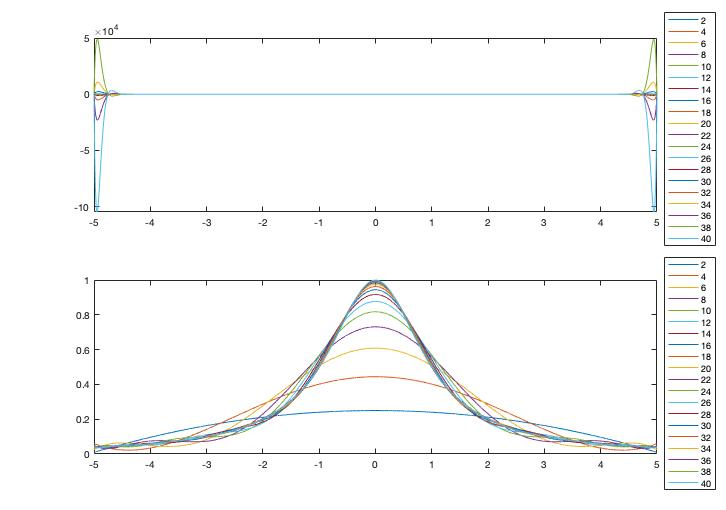
\includegraphics[width=\textwidth]{Chapter-4/Exercise-19/plot.jpg}
	\caption*{Polinomio di Lagrange con n° di ascisse $[2,4,6,8,..,40]$}
\end{figure}
Nelle seguenti tabelle è riportato come varia la \textit{costante di Lebesgue} $\Lambda$, al variare del grado \textit{n} del polinomio e si può notare come la crescita sia \textit{esponenziale}, per $n\rightarrow\infty$, prendendo in cosiderazione \textit{ascisse equidistanti}:\\\
\begin{table}
	\begin{center}
		\caption{Costante di Lebesgue con ascisse equispaziate}
		\begin{tabular}{|c|c|}
			\hline
			$n$ & $\Lambda$ \\
			\hline
			$2$  & $1.250000000000000$ \\ 
			$4$  & $2.207824277504000$ \\ 
			$6$  & $4.549341110838356$ \\ 
			$8$  & $10.945005461386041$ \\ 
			$10$ & $29.898141093562188$ \\ 
			$12$ & $89.323735973507041$ \\ 
			$14$ & $2.831809493441890e+02$ \\ 
			$16$ & $9.342736404823136e+02$ \\ 
			$18$ & $3.170339307979169e+03$ \\ 
			$20$ & $1.097924392398584e+04$ \\ 
			$22$ & $3.866684343844037e+04$ \\ 
			$24$ & $1.378514896760509e+05$ \\ 
			$26$ & $4.964824917524024e+05$ \\ 
			$28$ & $1.802445465492321e+06$ \\ 
			$30$ & $6.592504744423425e+06$ \\ 
			$32$ & $2.430870357380395e+07$ \\ 
			$34$ & $8.978560703086898e+07$ \\ 
			$36$ & $3.348225693891219e+08$ \\ 
			$38$ & $1.249687039228850e+09$ \\ 
			$40$ & $4.678649708006595e+09$ \\ 
			\hline
		\end{tabular}
	\end{center}
\end{table}
\begin{table}
	\begin{center}
		\caption{Costante di Lebesgue con ascisse di Chebyshev}
		\begin{tabular}{|c|c|}
			\hline
			$n$ & $\Lambda$ \\
			\hline
			$2$  & $1.429872254730518e+00$ \\ 
			$4$  & $1.685135237733246e+00$ \\ 
			$6$  & $1.866863755668355e+00$ \\ 
			$8$  & $2.008324271512492e+00$ \\ 
			$10$ & $2.123677735937467e+00$ \\ 
			$12$ & $2.221698051371436e+00$ \\ 
			$14$ & $2.304741888790266e+00$ \\ 
			$16$ & $2.381233643402699e+00$ \\ 
			$18$ & $2.447573290086530e+00$ \\ 
			$20$ & $2.508706712856935e+00$ \\ 
			$22$ & $2.549521672833381e+00$ \\ 
			$24$ & $2.612618302290017e+00$ \\ 
			$26$ & $2.647525891619366e+00$ \\ 
			$28$ & $2.699620139181539e+00$ \\ 
			$30$ & $2.742631723381937e+00$ \\ 
			$32$ & $2.771163414194285e+00$ \\ 
			$34$ & $2.802963771799375e+00$ \\ 
			$36$ & $2.839252073343268e+00$ \\ 
			$38$ & $2.869838999732480e+00$ \\ 
			$40$ & $2.909700595498265e+00$ \\ 
			\hline
		\end{tabular}
	\end{center}
\end{table}
